

The given system of inequality can be written in matrix form as
\begin{align}
    \myvec{-4 & -3 \\ -2 & 1 \\ 1 & 0 \\ 1 & 0 \\ 0 & 1}\vec{x} \succeq \myvec{-60\\0\\3\\0\\0}
\end{align}
which can be further simplified into 
\begin{align}
    \myvec{-4 & -3 \\ 1 & 0 \\ 0 & 1}\vec{x} \succeq \myvec{-60\\3\\6}
\end{align}

Let the surplus vector be
\begin{align}
    \vec{u} &= \myvec{u_1\\u_2} \succeq 0
\end{align}

\begin{enumerate}
    \item 
    \begin{align}
        \myvec{-4 & -3 \\ 1 & 0}\vec{x} &\succeq \myvec{-60 \\ 3}
        \\
        \implies  \myvec{-4 & -3 \\ 1 & 0}\vec{x} &= \myvec{-60 \\ 3} + \vec{u}
    \end{align}
    resulting in 
    \begin{align}
        \vec{x} &= \myvec{-4 & -3 \\1 & 0}^{-1}\myvec{-60 \\ 3} + \myvec{-4 & -3 \\1 & 0}^{-1}\vec{u}
        \\
        \implies \vec{x} &= \myvec{3 \\16} + \myvec{0 & 1\\ \frac{-1}{3} & \frac{-4}{3}}\vec{u}   \label{ineq/2/57eq1}
    \end{align}

    \item 
    \begin{align}
        \myvec{-4 & -3 \\ 0 & 1}\vec{x} &\succeq \myvec{-60 \\ 6}
        \\
        \implies  \myvec{-4 & -3 \\ 0 & 1}\vec{x} &= \myvec{-60 \\ 6} + \vec{u}
    \end{align}
    resulting in 
    \begin{align}
        \vec{x} &= \myvec{-4 & -3 \\0 & 1}^{-1}\myvec{-60 \\ 6} + \myvec{-4 & -3 \\0 & 1}^{-1}\vec{u}
        \\
        \implies \vec{x} &= \myvec{\frac{21}{2} \\6} + \myvec{\frac{-1}{4} & \frac{-3}{4}\\ 0 & 1}\vec{u} \label{ineq/2/57eq2}
    \end{align}
\end{enumerate}

Now,solution region which is common to regions of eq. \eqref{ineq/2/57eq1} and eq. \eqref{ineq/2/57eq2},is given by

\begin{align}
    \boxed{\vec{x} = \myvec{3 \\ 6}+\myvec{0 & 1\\\frac{1}{12} & \frac{-13}{12}}\vec{u}}
\end{align}


\begin{figure}[!ht]
\centering
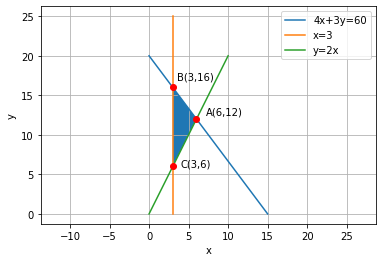
\includegraphics[width=\columnwidth]{solutions/su2021/2/57/Figures/Figure11_1.png}
\caption{Solution Region}
\label{ineq/2/57fig:fig1}	
\end{figure}

% \numberwithin{figure}{section}
% \begin{figure}[!ht]
% \centering
% 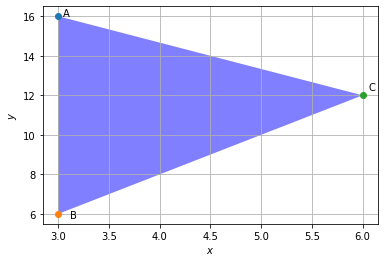
\includegraphics[width=\columnwidth]{Figure11_2}
% \caption{Magnified Solution Region}
% \label{ineq/2/57fig:fig2}	
% \end{figure}




%\end{document}
